%Thus far in this work a solution to simplify and automate design the process of all digital PLL loop filter designs comprised of (1) an automated loop filter optimization and design engine, and (2) a discrete-event, time domain PLL simulator to evaluate the designed filters with full time-discretization and quantization nonlinearity effects. I
In this discussion, the performance of the implemented design will first be analyzed via comparison to a theoretically calculated jitter limit, and current state of art. Small area and low power PLLs are considered for reference. Later, identified areas of improvement within the presented design are discussed.

\subsection{Radio System Performance}
	For the specified radio system, are reqs met? Due to 1/3 subharmonic, CNR at at 816 MHz is 1/9 that at 2.448 GHz. Are specs met???

\subsection{Performance Limit for Ring Oscillator BBPD PLLs with PI-controllers}\label{sec:fomjit_limit}
	In the case of a perfect ring oscillator PLL, all components would be noiseless and consume minimal possible energy. In the case of an ADPLL, the consideration of power can be divided between logic and oscillator. In the case of logic, the theoretical energy limit for switching of a logical level of a gate equates to $E_s = \ln(2) k_B T$, \cite{Lundstrom2006}. With a reference frequency of $f_{ref}$, and $N$ gates and digital, the minimum possible power expenditure from digital components of PLL is in equation \ref{eq:min_sw_energy}. This assumes the worst case scenario where all gates switch every cycle.
	\begin{equation}\label{eq:min_sw_energy}
		P_{min,digital} = Nf_{ref}\ln(2) k_B T
	\end{equation}
	At 300 K, the design considered in this work having complexity N $\approx$ 1000, and $f_{ref}$ = 16 MHz, yields a \textit{theoretical} consumption of 66 pW, practically zero. Infact, it is found \textit{theoretically} that the one can operate 242 thousand gates at 1 GHz and consume only 1 $\mu$W of power. Following these findings, and considering total PLL operating power on the regime of 1 $\mu$W, it has been assumed here that the theoretical power limit for digital components of an ADPLL is practically zero. In the case of a ring oscillator, however, power may not be scaled to zero as with logic. This is due to the fundamental relationship between oscillator power and phase noise, as discussed in section \ref{sec:ro_pn_limit}. Therefore, it is now asserted that an optimal (AD)PLL will expend all of its power in its oscillator. Analyzing the case presented in this work of a BBPD and PI-controller based PLL, it was determined that the expected value of total phase noise is in equation \ref{eq:optimal_pn_pow}. Using the theoretical limit of ring oscillator phase noise in equation \ref{eq:ro_pn}, the result of equation \ref{eq:min_pibbpdpll_pn} provides the minimum achievable PI-controller BBPD PLL phase noise.
	\begin{equation}\label{eq:min_pibbpdpll_pn}
		\sigma_{\Phi_{n,opt}}^2 = 74.79376\cdot \frac{\mathcal{L}_{min}(f)f^2}{f_{ref}} = 74.79376\cdot  \frac{7.33 k_B T f_{osc}^2}{f_{ref}P_{DC}}
	\end{equation}

	 This result can be converted into RMS jitter, with $\sigma_{\Phi_{n}} = 2\pi f_{osc}\sigma_{j_t}$, yielding equation \ref{eq:min_pibbpdpll_jit}.
	\begin{equation}\label{eq:min_pibbpdpll_jit}
		\sigma_{j_t}^2 = 74.79376\cdot  \frac{7.33 k_B T}{(2\pi)^2f_{ref}P_{DC}}
	\end{equation}


	  Using the FOM$_{jitter}$ expression in equation \ref{eq:ro_fom_limit}, it is seen that the theoretical limit for PLL FOM this class of PLL is in equation \ref{eq:ro_fom_jit_limit}. Noting the dependence on reference frequency, with $f_{ref}$=16 MHz at 300 K, this is -234.4 dB. Equation \ref{eq:ro_fom_jit_fom_pn} provides the general expression for FOM$_{jitter}$ limit provided an an oscillator FOM$_{pn}$ value. It should be noted that the only way to improve jitter FOM in the proposed architecture is to reduce temperature, increase frequency, or improve oscillator FOM (that is, use a resonant oscillator, such as an LC oscillator).
	\begin{equation}\label{eq:ro_fom_jit_limit}
		\textnormal{FOM}_{\textnormal{jitter,min}} = 10\log_{10}\left(\frac{\sigma_{t_j}^2}{(\textnormal{1 s})^2}\cdot\frac{P_{DC}}{\textnormal{1 mW}}\right) =  10\log_{10}\left( 74.79376\cdot  \frac{7.33\times 10^3 k_B T}{(2\pi)^2f_{ref}} \right)
	\end{equation}
	\begin{equation}\label{eq:ro_fom_jit_fom_pn}
		\textnormal{FOM}_{\textnormal{jitter,min}} = \textnormal{FOM}_{pn} + 10\log_{10}\left(\frac{74.79376}{(2\pi)^2 f_{ref}} \right)
	\end{equation}

\subsection{State of art}
In order to form a comparison to the current state of art for ultra low power PLLs, a wide search of  literature was undertaken, and data from relevant PLL designs were collected into table \ref{tab:state_of_art}. Specific criteria for this search were power consumption below 1 mW, publication within 2 years of this work, similar oscillation frequency, and preference to ring oscillator designs implementing integer-N architectures. Filtering in this manner has resulted in a curated selection of 5 highly comparable designs to the one of this work.

Analyzing FOM$_{jitter}$, this work is on the lower end of being state of art, achieving -226.5 dB, where the observed range was [-236.8,-226.1] dB for the surveyed works. Using the theoretical limit for FOM$_{jitter}$ in this topology derived in \ref{sec:fomjit_limit}, the best achievable value of FOM$_{jitter}$ possible with this work using a ring oscillator is -234.4 dB (at 300K and $f_{ref}$ = 16 MHz). Adding a penalty for consuming power in non-oscillator components (20 $\mu$W of 100 $\mu$W power budget) results in a 1 dB reduction from the optimal FOM, and the oscillator performing 5 dB worse than theoretically obtainable -165.2 dB yields a total penalty of 6 dB. Thus the realistic best case result in this design is therefore -228.4 dB, which justifies the positioning on the low end of FOM$_{jitter}$ for comparable designs. In equation \ref{eq:ro_fom_jit_fom_pn}, oscillator FOM is seen to be improved with increasing reference frequency. In this work, however, a higher reference freqency is not an option, as this design was constrained with a 32 MHz reference frequency, and this must be divided to 16 MHz to achieve an integer ratio to the synthesized frequency of 2448 MHz. If it were possible to increase the reference frequency, for example to 200 MHz as in \cite{Xiang2020}, the theoretical FOM$_{jitter}$ then is extended to -245.4 dB, or -239.4 dB penalized, bringing it to be far competitive with the other works. As a general statement, the FOM$_{jitter}$ of this work is necessarily limited by the design constraints imposed on the design.

In terms of oscillator perfomance, this design comes out ahead of all others in power, utilizing only 80$\mu$W. The next closest work in oscillator power is that by Liu'19 \cite{Liu2019}. That design uses an LC VCO with a SSB phase noise of -107 dBc/Hz at 1 MHz for 2.46 GHz frequency, yielding an oscillator FOM of -184.5 dB. The oscillator is only a single stage differential LC oscillator, consuming 107 $\mu$W. Practically, the PLL of this work is required to generate quadrature signals, so the non-quadrature 107 $\mu$W of that work should be doubled, i.e. to 214 $\mu$W, to estimate power consumption for quadrature phase generation. A new oscillator FOM of -181.5 is achieved, which is 21.5 dB improved over the -160 dB achieved in this work. It is not expected the remaining works are substantially better than this work in terms of phase noise, due to them being ring oscillator based, coupled with the theoretical limit of -165.2 dB for FOM phase noise at 300 K. Based purely on oscillator phase noise values, and the prediction for PI-controller BBPD-PLL FOM$_{jitter}$ in equation \ref{eq:ro_fom_jit_fom_pn}, the LC-based PLL should be expected to achieve \textit{atleast} 21.5 dB better FOM$_{jitter}$ than this work. However, this is not completely observed, Liu only reports -236.8 dB, an improvement of 10.3 dB over this work, the discrepency is probably due to the FLL architecture used in that work. It appears that the oscillator core from Liu's work, coupled with the PLL topology of this work, would yield a FOM$_{jitter}$ of -248.0 dB, substantially better than that demonstrated in either work. It is a question, perhaps for future work, to determime if an LC oscillator core can be used satisfactorily with the topology of this work for the needs of wake up receivers. Issues croping up related to the LC oscillator may prove challenging due to non-instaneous start up, and inability to reset phase to align to a clock edge instantly, which may overall lead to instability with the BBPD-PLL and or slow lock times. 

In regards to implementation area, this work is favorable compared to the other assembled designs, only beat in area by 30\% by a PLL built in 5nm technolgy by Liu'20 \cite{Liu2020}. This should be expected due to substantially smaller devices in 5nm versus the 22nm in this work. The LC based design by Liu'19 achieved an area 49x of this work, which was limited by integration area needed by the resonant LC circuit to have sufficiently high-Q. The analog designs also came close in area. One implemened by Zhang'19 \cite{Zhang2019} in 40 nm technology came close with only 1.746x greater area.

Concerning analog versus digital implementation, the two analog ring-oscillator PLL designs (Zhang'19 \cite{Zhang2019} and Xiang'20 \cite{Xiang2020}) are comperable in terms of FOM, however, power is not seen to scale as low as this work. Both designs also employ higher reference frequencies than here, being 100 MHz \cite{Zhang2019} and 200 MHz \cite{Xiang2020}, which is expected to help reduce phase noise contribution from the oscillator significantly, as much higher loop bandwidth can be used, bringing down the in-band phase noise level. The analog designs discussed here are both phase-frequency detector and charge pump based, whose dynamics are linear \cite{Razavi2020}, in comparison to the BBPD that is inherently nonlinear due to its detector characteritics. As seen in this work, BBPD designs have some undesirable consequences which increase phase noise contributions, and this can be mitigated to some extent with linearized designs employing PFD and CP loop filters. It is expected that analog implementation will, however, introduce extra analog noise into the loop. It is possible to implement a PFD with CP loop filter digitally to remove these noise sources, as Palaniappan'18 \cite{Palaniappan2018} does, to take advantage of the transfer function linearity. In that work, comperable FOM (-226.1 dB) was seen to this work, albeit at a lower output frequency of circa 400 MHz. The PFD approach is not necessarily better, as in practice, equal performance in terms of total jitter is achievable with BBPD and charge pump designs according to \cite{xu_abidi_2017}. Furthermore, implementation complexity is higher for a PFD, nominally requiring two D flip flops and an AND gate \cite{Razavi2020}, whereas a BBPD is as simple as a single D flip flop. Thus, when scaling for minimum power, lower power should be achievable with a BBPD as it is simpler. Overall, it does not appear that analog implementation pose any significant advantages based upon existing works in the ultra low power sub-1mW regime when considering the design of a 100$\mu$W PLL. Rather, digital implementation are more favorable due to lower sensitivity to PVT variation, as the bulk of the circuits are digital.

In terms of lock time, highly favorable performance was seen in the analog design of Xiang, with circa 0.2 $\mu$s. However, a high reference frequency of 200 MHz is used, or equivalently 20 reference cycles. 20 reference cycles in this work is 1.25 $\mu$s, so it is more comperable to this work. Inspecting the the best FOM result of the table (Liu'19), an extremely long lock time is seen due to using a frequency locked loop approach requiring long calibration periods to adjust the frequency, in upwards of 120$\mu$s (1200 cycles at 10 MHz). This FLL approach does not appear viable for fast start of needs in WUR.

Two of the reviewed papers presented interesting comparison figures for (a) PLL FOM versus power consumption, in figure \ref{fig:fom_v_pow}, and (b), FOM versus implementation area, in figure \ref{fig:fom_v_area}. The works that the figures were published in are from 2019 and 2020 respectively. With the PLL of this work having a power consumption of 100 $\mu$W, a FOM$_{jitter}$ of -226.5 dB, and area of 0.0051 mm$^2$, it is seen that this design lands off the chart, beyond the suggested FOM trend line in power versus FOM, and lands in a comparable position with other state of art design in terms of FOM versus area. Based on this comparison, it is concluded that this work is a leading design in terms of power consumption, and is also state of art in area of implementation.


	\begin{figure}[htb!]
	    \centering
	    \begin{subfigure}{0.5\textwidth}
	        \centering
	        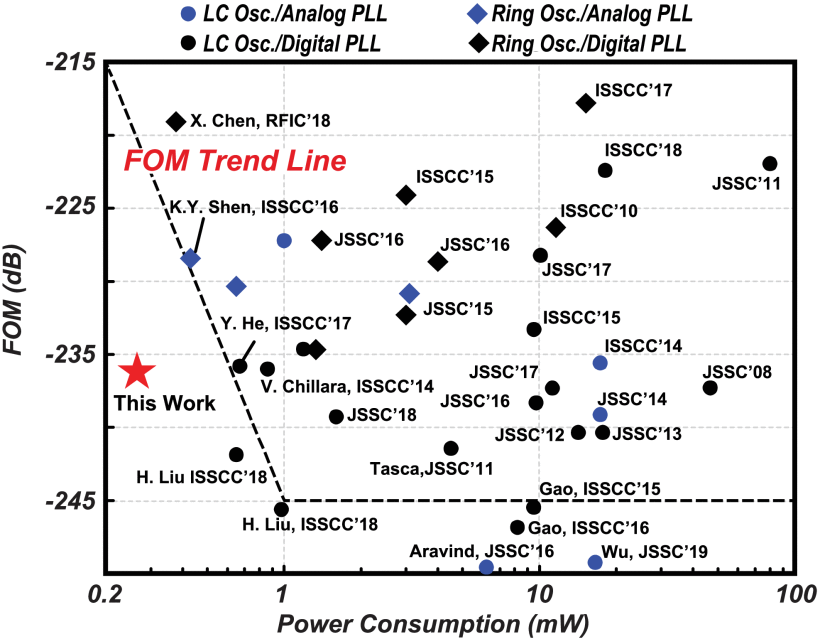
\includegraphics[width=1\textwidth, angle=0]{./figs/liu24-fom}
	        \caption{ }
	        \label{fig:fom_v_pow}
	    \end{subfigure}%
	    \begin{subfigure}{0.5\textwidth}
	        \centering
	        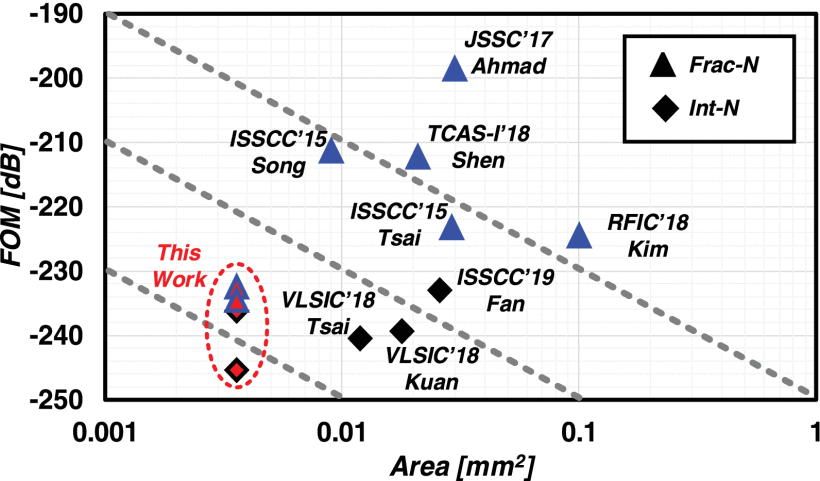
\includegraphics[width=1\textwidth, angle=0]{./figs/liu_5nm}
	        \caption{ }
	        \label{fig:fom_v_area}
	    \end{subfigure}
	    \caption{\textbf{(a)} FOM$_{jitter}$ versus power from \cite{Liu2019} (JSSC 2019), \textbf{(b)} FOM$_{jitter}$ versus area from \cite{Liu2020} (SSCL 2020). Note, "This work" refers to that described in the source papers.}
	    \label{fig:fom_charts}
	\end{figure}


	% \FloatBarrier
	\begin{table}[h!]
		\centering
		\def\arraystretch{1.5}		
		\setlength\arrayrulewidth{0.75pt}
		\setlength{\tabcolsep}{0.5em} % for the horizontal padding
		\begin{tabular}{|>{\centering}m{0.2\textwidth}?>{\centering}m{0.1\textwidth}?>{\centering}m{0.11\textwidth}|>{\centering}m{0.1\textwidth}|>{\centering}m{0.1\textwidth}?>{\centering}m{0.11\textwidth}|>{\centering\arraybackslash}m{0.1\textwidth}|}
			\hline 
			\rule[-1ex]{0pt}{2.5ex} \cellcolor{gray!40}\textbf{Parameter} & \cellcolor{gray!40}\textbf{This Work} & \cellcolor{gray!40}\textbf{JSSC'19 Liu} \cite{Liu2019} & \cellcolor{gray!40}\textbf{{\footnotesize NORCHIP'18 Palaniappan} }\cite{Palaniappan2018} & \cellcolor{gray!40}\textbf{SSCL'20 Liu} \cite{Liu2020} & \cellcolor{gray!40}\textbf{2019 Zhang} \cite{Zhang2019} & \cellcolor{gray!40}\textbf{CICC'20 Xiang} \cite{Xiang2020} \\
			\hline 
			\rule[-1ex]{0pt}{2.5ex} \textbf{Analog/Digital} & Digital  & Digital  & Digital & Digital & Analog & Analog \\
			\hline 
			\rule[-1ex]{0pt}{2.5ex} \textbf{Int-N/Frac-N} & Int-N  & Frac-N  & Int-N & Int-N & Int-N & Int-N  \\
			\hline 
			\rule[-1ex]{0pt}{2.5ex} \textbf{Architecture} & BB-PLL\tablefootnote{BBPD PLL} & FLL + ODZ\tablefootnote{Out of deadzone detector}  & {Digital CP-PLL\tablefootnote{Charge Pump PLL}} & IL-PLL\tablefootnote{Injection-locked PLL} & CP-PLL & CP-PLL \\
			\hline 
			\rule[-1ex]{0pt}{2.5ex} \textbf{Process} & 22nm & 65nm & 40nm & 5nm & 40nm & 22nm \\
			\hline 
			\rule[-1ex]{0pt}{2.5ex} \textbf{Osc. Type} & RO & LC & RO & RO & RO  & RO \\
			\hline 
			\rule[-1ex]{0pt}{2.5ex} \textbf{Detector} & BBPD & ODZ & PFD\tablefootnote{Phase-frequency detector} & Sampling & PFD & PFD\\
			\hline
			\rule[-1ex]{0pt}{2.5ex} \textbf{Area [mm$^2$]} & 0.0051 & 0.25 & 0.0186 & 0.0036 & 0.00873 & 0.015 \\
			\hline 
			\rule[-1ex]{0pt}{2.5ex} \textbf{Power [$\mu$W]} & 100 & 265 & 270.5 & 440 & 170  & 682 \\
			\hline 		 
			\rule[-1ex]{0pt}{2.5ex} \textbf{f$_{ref}$ [MHz]} & 16 & 10 & - & 40 & 100 & 200 \\
			\hline 
			\rule[-1ex]{0pt}{2.5ex} \textbf{f$_{osc}$ [GHz]} & 0.816 & 2.1-3.1 & 330-470 & 1.0 & 1.6 & 3.2 \\
			\hline 
			\rule[-1ex]{0pt}{2.5ex} \textbf{Osc. Stages (N$_{stg}$)} & 6 & 1 & 8 & - & 3 & - \\
			\hline 
			\rule[-1ex]{0pt}{2.5ex} \textbf{f$_{osc}$ $\times$ N$_{stg}$} [GHz] & 4.896 & 2.1-3.1 & 2640-3760 & - & 4.8 & - \\
			\hline 	
			\rule[-1ex]{0pt}{2.5ex} \textbf{Osc. Power [$\mu$W]} & 80 & 107 & - & 398 & - & 225 \\
			\hline 		
			\rule[-1ex]{0pt}{2.5ex} \textbf{Jitter [ps$_{RMS}$]} & 15.1  & 2.8 & 9.53 & 2.34 & 8.3 & 2.3 \\
			\hline 			
			\rule[-1ex]{0pt}{2.5ex} \textbf{$\textnormal{FOM}_{\textnormal{jitter}}$ [dB]} & -226.5  &  -236.8 & -226.1 & -236.2 & -229.3 & -234.3 \\
			\hline 		
			\rule[-1ex]{0pt}{2.5ex} \textbf{Lock-time [$\mu$s]} & $\leq$ \hl{X} & $\leq$ 120  & - & - & - & 0.2 \\
			\hline 			
		\end{tabular} 
		% \caption{Assigned specifications for branch line hybrid design.}
		% \label{asgn_specs}
		\caption{PLL parameters determined from filter design and optimization process for minimum phase noise with BBPD.}
		\label{tab:state_of_art}
	\end{table}  



	% \begin{figure}[htb!]
	% 	\center\includegraphics[width=1.0\textwidth, angle=0]{figs/x.pdf}
	% 	\caption{Transient simulation of optimal design.}
	% 	\label{fig:des_ex_trans}
	% \end{figure}
	% \FloatBarrier

	% \begin{figure}[htb!]
	% 	\center\includegraphics[width=1.0\textwidth, angle=0]{figs/x.pdf}
	% 	\caption{Variation Simulation for KDCO.}
	% 	\label{fig:var_lock}
	% \end{figure}
	% \FloatBarrier

	% \begin{figure}[htb!]
	% 	\center\includegraphics[width=1.0\textwidth, angle=0]{figs/x.pdf}
	% 	\caption{Phase noise.}
	% 	\label{fig:Simulated phase noise.}
	% \end{figure}
	% \FloatBarrier

	% stability criteria - Jurys' stability criteria abs(a0) l.t. a2 for second order z-transfer \cite{xiu_li_meiners_padakanti_2004}
	% - Not phase margin based in optimization, can make stable by using stable choice of PI controller (two poles only) - poles should be in unit circle...
\FloatBarrier


\subsection{Areas of improvement}
	\subsubsection{LC Oscillator}
	Based on the 100 $\mu$W power range LC-oscillator of \cite{Liu2019}, it is expected that on the order of 20 dB of oscillator phase FOM improvement is achievable over ring oscillators in the power domain of circa-100 $\mu$W. Based on equation  \ref{eq:ro_fom_jit_fom_pn}, 20 dB of phase noise improvement should yield 20 dB in the jitter FOM, which characterizes RMS phase noise per unit power. It is therefore suggested to explore extension of this work to LC-based oscillators. It is unknown, however, if limitations imposed in LC-oscillator start up time, and power requirements of supporting circuitry for such an oscillator will be prohibitive in a PI-controller BBPD-PLL.

	\subsubsection{Coarse calibration}
	The coarse calibration scheme implemented is capacitor based, and does not provide robust enough tuning in the presence of process and voltage variation. The coarse implementation of this work allows for approximately 15\% fractional tuning range, where as standard deviation the simulated oscillator variance due to process variation under fixed biasing is 4.2 \% of the oscillator frequency. This results in coverage of $\pm$1.78$\sigma$ of the sample variance from the mean, or a yield of 92.5\% under ideal biasing. However, under non ideal biasing conditions, extra deviation of the oscillator frequency is inherent. It was observed from simulation that the oscillator frequency deviates by 2.588 MHz/mV of extra bias, or 0.3\% of the oscillator frequency per mV. A $V_{DD}$ offset of only 47.3 mV (6\% of 0.8V) to shift the oscillator by 15\%, enought that there is no expectation that the coarse calibration can correct the frequency range. 

	The current capacitor-based coarse calibration is limited due to the loading it exerts on the ring oscillator core. For a greater tuning range, a larger bank work would be required, however it was found during the design process that obtaining the correct frequency range under constrained power with acceptable phase noise was not possible with a larger capacitor bank. A highly viable solution to this problem is to use tuning of the supply voltage to implement coarse tuning, and to forgo the capacitor tuning bank all together. Removal of the capacitor bank will reduce oscillator core loading, thus increasing frequency of the oscillator. Longer channel lengths could be used in the oscillator core (again reducing frequency), to improve phase noise performance. Such a change would require implementation of a digitally tunable voltage regulator for the oscillator core, with tight regulation of supply voltage. Requirement of tight regulation of the supply is paramount due to the high frequency gain of the oscillator with supply tuning (again 2.588 MHz/mV, or 0.3\%/mV). Design of such a regulator within the PLL power requirements is possibly a daunting endeavor, and has been considered outside of the current scope of this work, as a possible future area of improvement.

	\subsubsection{Subharmonic oscillator}
		The usage of a 1/3 subharmonic oscillator as in this work is possibly undesirable in some regards for application to radio receiver design. This design choice pushes additional circuit complexity into receiver circuits, which must be designed to achieve full rate sampling by edge combining the 12 oscillator phases resulting from the 6-stage, 1/3 sub-harmonic oscillator. It is therefore probable that topological improvements for achieving full frequency operation of this PLL design for radio applications is a possible area of improvement. The removal of the capacitive tuning bank in the oscillator core, and utilization of supply tuning may allow for higher operating frequency for such an improvement to be realized.

	\subsubsection{CDAC switching noise}	
		It has been observed in the implemented CDACs that transient spikes occur in the DAC output during changing of the input code, as demonstrated in figure \ref{fig:dac_sw_noise}. This is a result of differing RC constants of the different switch and capacitor combinations.  The small RC constant switch and capacitor combinations will settle very fast, causing an inital rising/falling portion of a spike to be seen in the DCO ouput. The larger capacitor and switch combinations will settle delayed in time, causing the spike to subside and the output to settle to the desired value. The DCO spikes, while short in duration, are expected to have a contribution to increasing phase noise of the oscillator. An area of improvement in future is to reduce this spiking, through more careful design of the switch and capacitor combinations. 
		\begin{figure}[htb!]
	        \centering
	        \includegraphics[width=0.65\textwidth, angle=0]{example-image}
		    \caption{Noise tranients in DAC output during switching.}
		    \label{fig:dac_sw_noise}
		\end{figure}

	\subsubsection{Ignored Flicker Noise}
	In this work, only noise components proportional to $1/f^2$ were considered for purposes of PLL optimization. $1/f^2$ noise components were specifically paid attention due to being a fundamental component of ring oscillator phase noise \cite{Navid2005}, whereas flicker ($1/f$) components are dependent primarily on device characteristics. To simplify derivation, consideration of the fundamental $1/f^2$ noise components were the sole focus of optimization. In cases where flicker noise is significant, it may be meaningful to derive optimization theory including flicker noise effects.

	\subsubsection{Synchtonous Counter}
	Does not work well - low resoltion, suffers from the fact that phase is always rounded down in effect. Can end up with count near steady state rapidly toggling, which can affect operation of BBPD (often possible that BBPD mode locks to not desired frequency due to SCPD behavior)

\FloatBarrier
% \normalsize